\documentclass[8pt, a4paper]{article}
\usepackage{geometry}
\geometry{total={170mm, 257mm},left=20mm, top=20mm}
\usepackage{graphicx}
\usepackage{float}
\usepackage{hyperref}
\usepackage{listings}

\begin{document}
\setlength \topmargin{-1in}
\title{\textbf{Software Engineering for Distributed and Interactive Systems.}}
\author{\textbf{James Ravenhill}}
\date{}
\maketitle

\section{Introduction} 

The main outcome at the beginning of the project was to create a simple and easy to used piece of software which allows the user to control the buggy without being too complex. Both the hardware and software have been an ongoing development based on feedback given through multiple tests, which a few friends generously took part in. The main objectives of the project are listed below but not limited to:

\begin{itemize}
	\item Reliability - Unreliable connection/data transfer is a disadvantage and creates more problems. This will be explained later in more detail.  
	\item  Multiple methods of communication - By using WiFi, Bluetooth, IR remote and PC. 
	\item Scalability - There should be no software problems while developing the increased load of sensor/capabilities of the buggy. 
	\item Maintainability - comments/documentation is clear to allow future developers to understand the project decisions as they happen. 
	\item Autonomous - The buggy has the ability to move in and out of an autonomous mode.  
\end{itemize}

In this document short snips of the main code will be used in explanations. The main raw code can be found in the submitted documents or on my $\href{https://github.com/james8268/Buggy}{Github}$ account.
 

\section{Design}
In terms of hardware design, the overall aesthetic is not very relevant. This being said, proper cable management and reducing the risk of damaging hardware was a great challenge due to the limited mounting points on the buggy. This challenge was overcome by using blue tac or Velcro to attach the hardware to the buggy without damaging the hardware in the process. 

\begin{figure}[H]
\centering
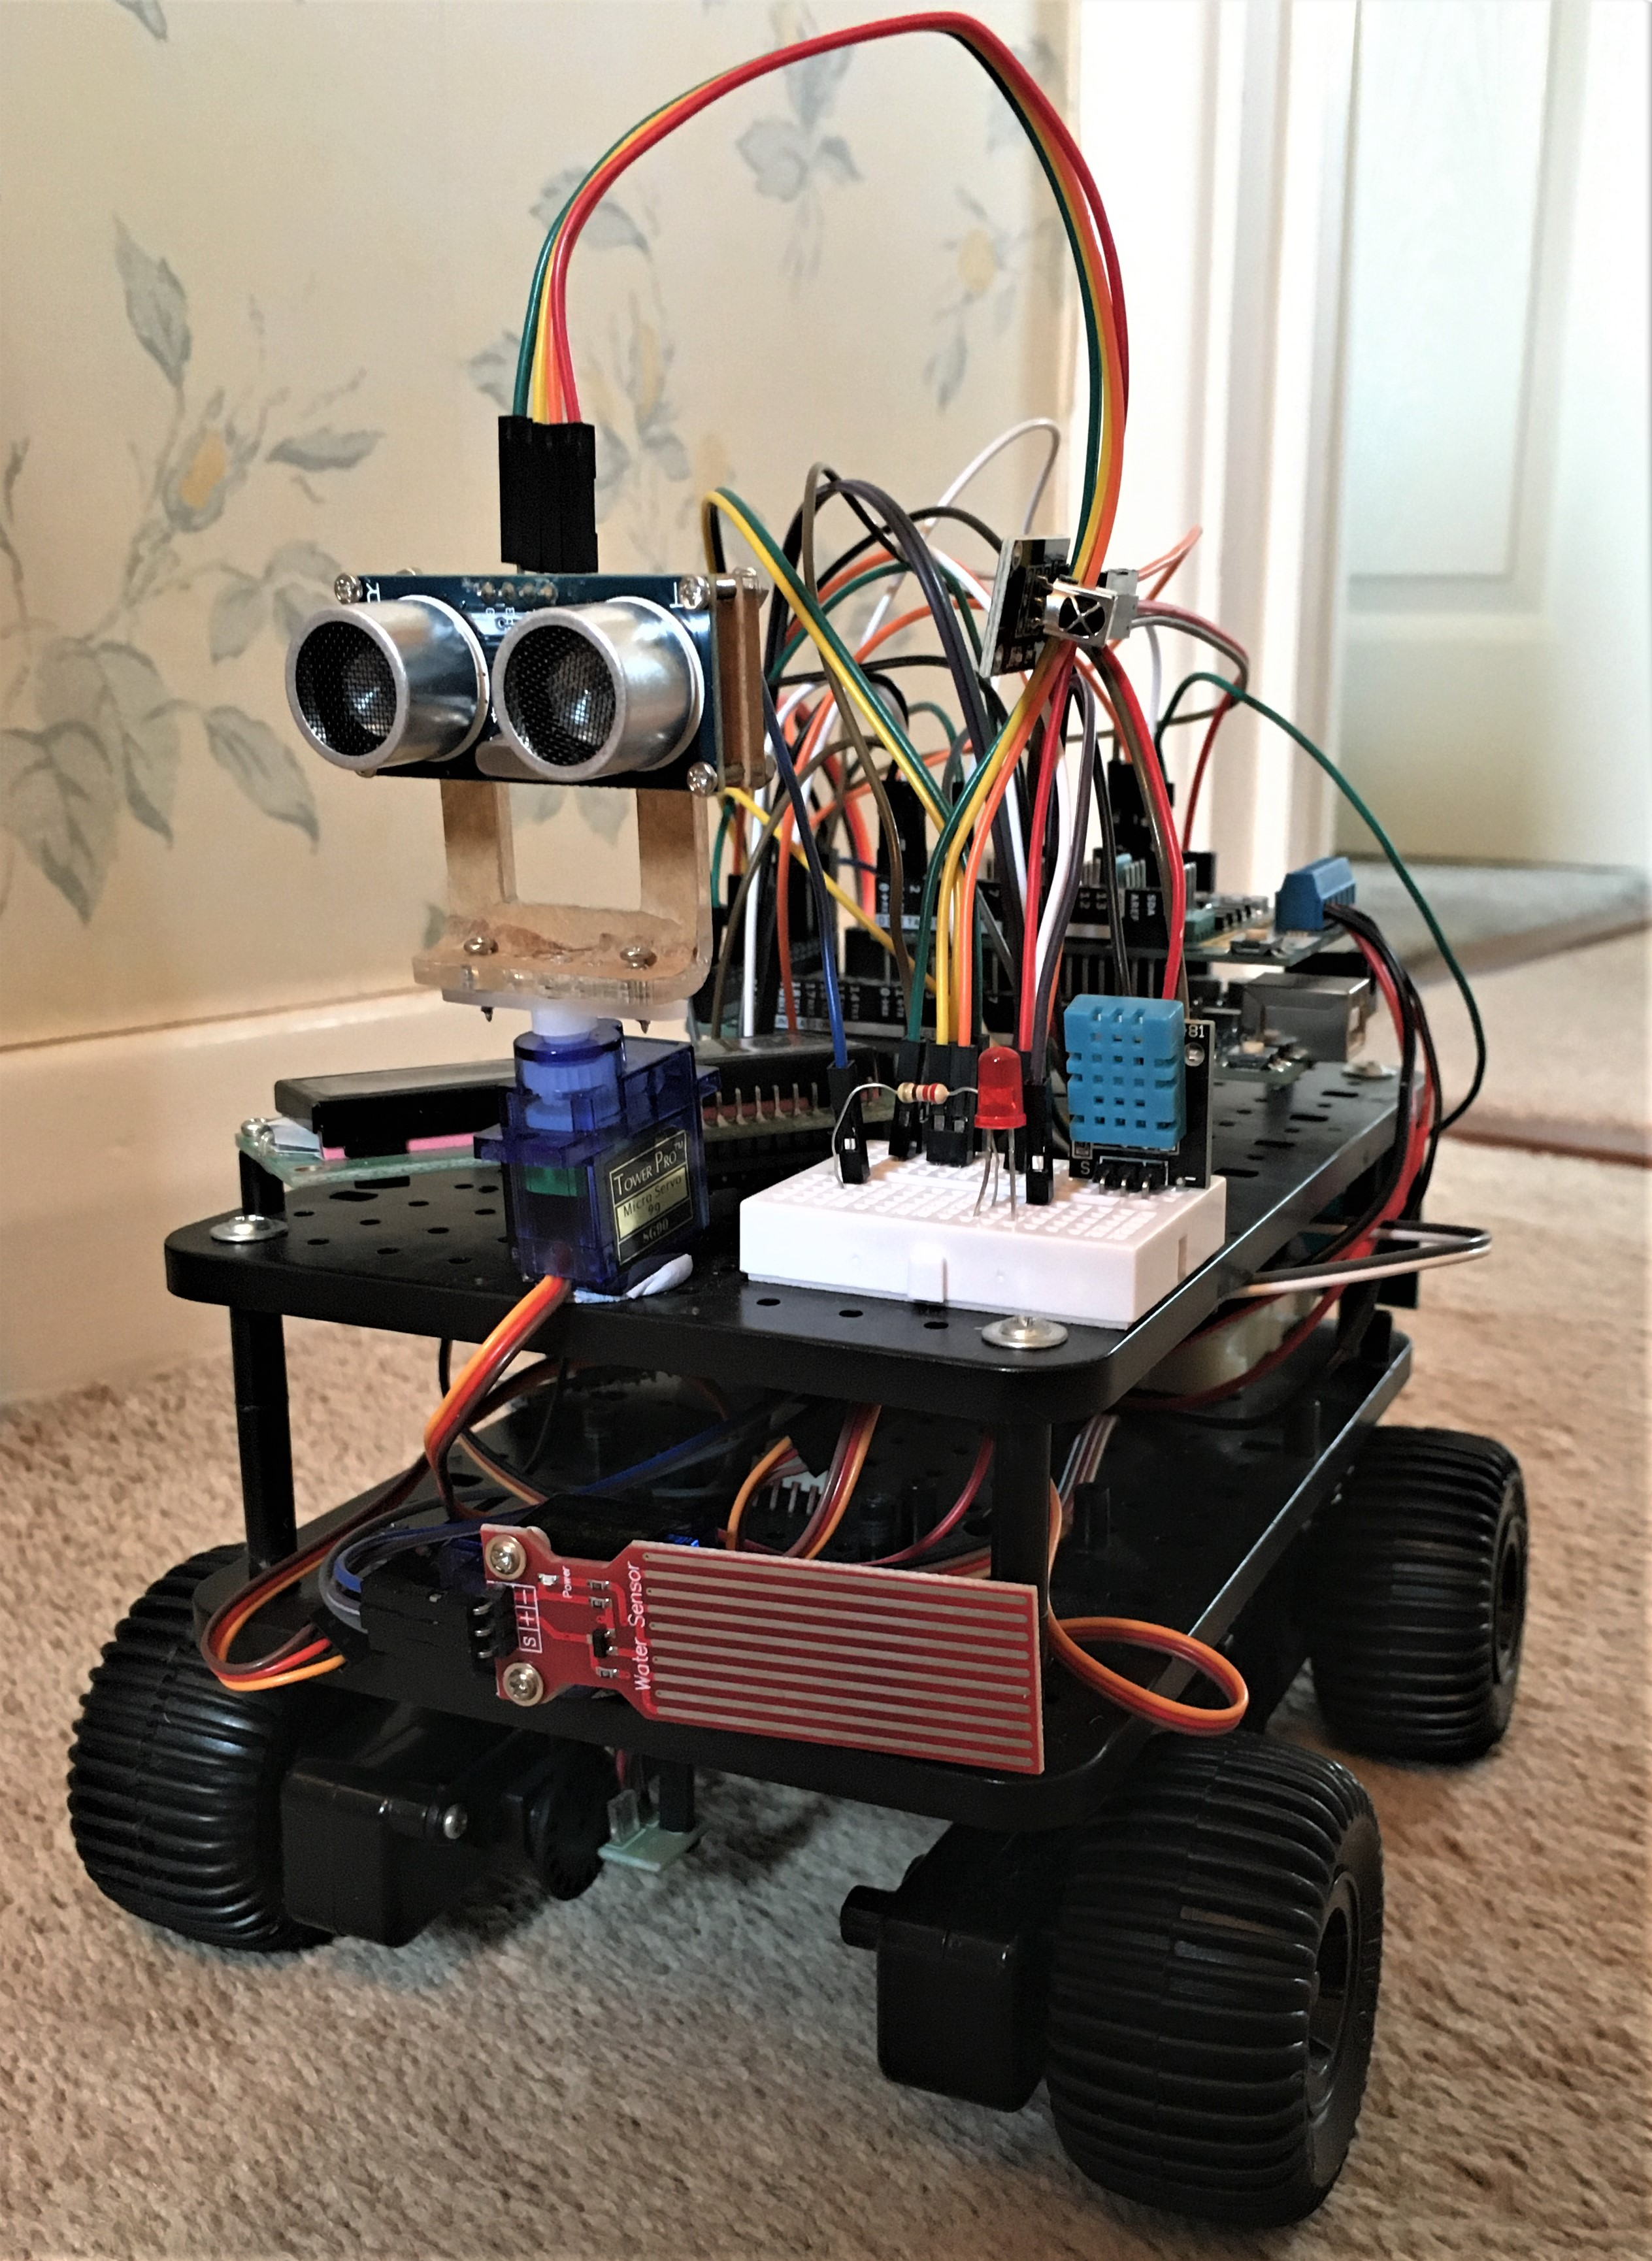
\includegraphics[height=4.0cm, width=5.0cm]{buggy_front}
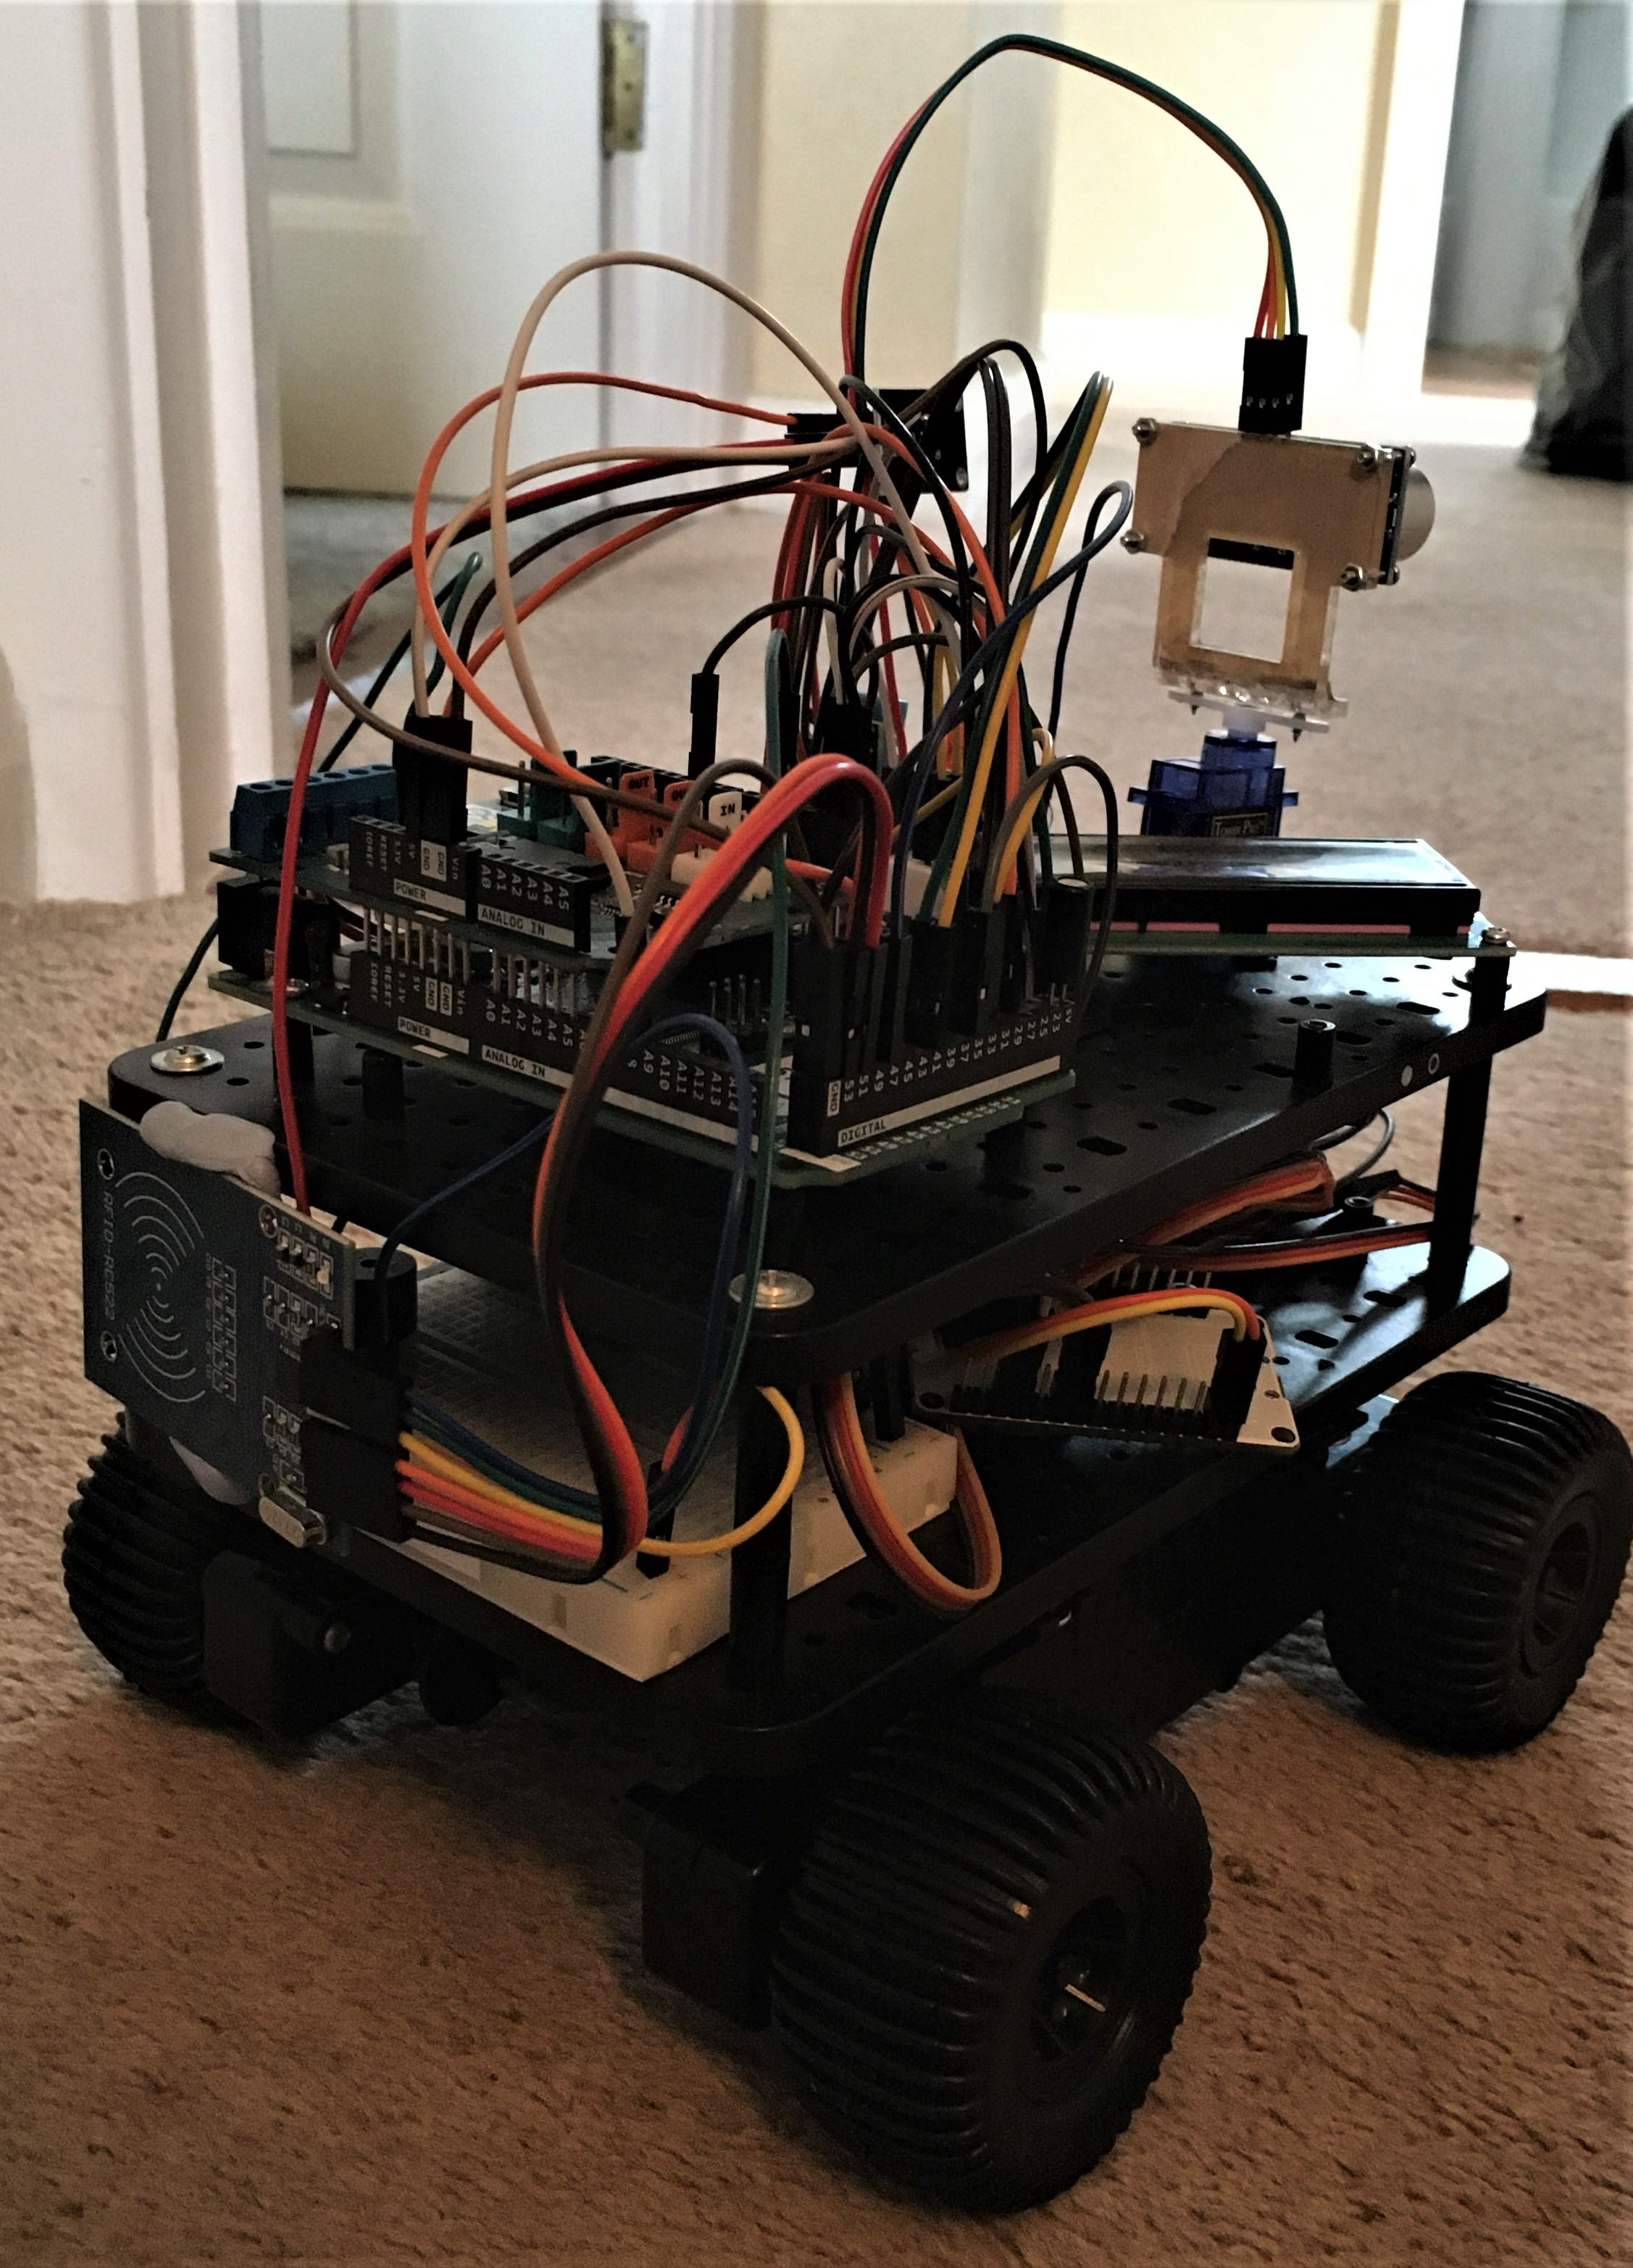
\includegraphics[height=4.0cm, width=5.0cm]{Buggy_rear}
\caption{Left: Image of Buggy from the front left corner.}
\caption{Right: Image of Buggy from rear right corner.}
\end{figure} 


Below are two images of the main schematic of the buggy and a general communications diagram. 


\begin{figure}[H]
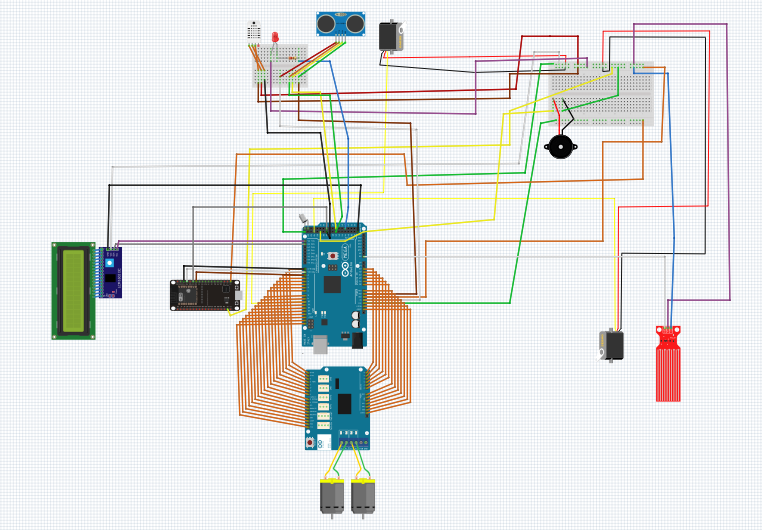
\includegraphics[height=5cm, width=7.0cm]{schematic}
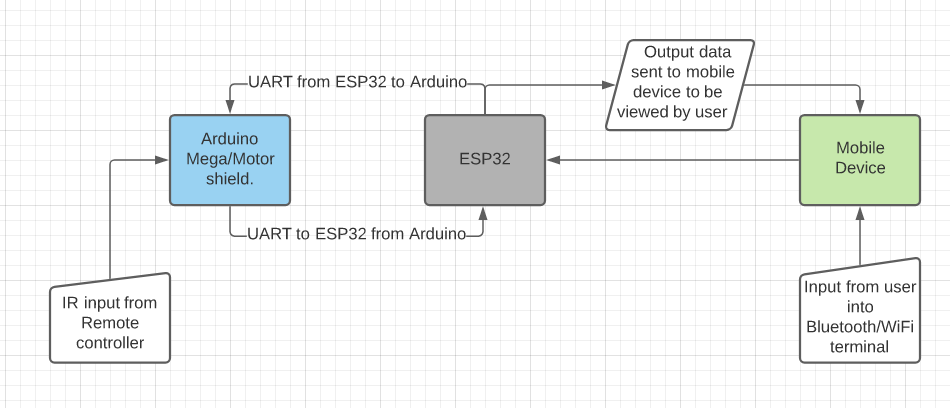
\includegraphics[height=5cm, width=7.0cm]{Arch}
\caption{Left: Schematic of Buggy.}
\caption{Right: Communication diagram of the Buggy}
\end{figure}

The software for the Arduino has been set up into header (.h) files and source code (.cpp) files where they are then called in the main code. There are many benefits to this such as the code is organised and tidy allowing future and current developers to debug with ease, addition of any new code can be easily integrated into the system and the code can be easily maintained. 

\begin{figure}[H]
	
\includegraphics[width=17cm]{tabs}
	\caption{Tabs for Arduino mega main code.}
\end{figure}

In Figure 4 you can see how the system communicates between source files. The main system that operates the buggy can not be accessed without first passing the RFID security tag challenge. Further development to encrypt data that is sent between the mobile device and ESP32 needs to be done, a attempt to create a rotation 13 encryption has been attempted but needs to be placed correctly within the architecture of the system. 

The Buggy can be controlled with various methods.
\begin{itemize}
	\item Bluetooth- The buggy can be controlled with a mobile device via Bluetooth. With this method the buggy can be used to its full potential and all functions are available, ithis includes influencing the direction the buggy moves, taking measurements and allowing the buggy to move around autonomously while avoiding obstacles. 
	\item WiFi- The buggy can also be controlled with a mobile device via WiFi. This method also allows the user to use the buggy to its full potential. 
	\item IR Remote- This works well when in close proximity to the buggy or when simultaneously using a mobile device to control the buggy. The limitation to this is that you can not control the buggy for its autonomous mode when using the IR remote.
	\item PC- The serial monitor can also be used to control the buggy, but like the IR remote the buggy can not be controlled autonomously with this method. 
	\item WiFi and Bluetooth- The ESP32 has a dual core CPU so Bluetooth and WiFi can be used on two separate mobile devices to control the buggy simultaneously.  
\end{itemize}	


\section{Implementation}

The software for the ESP32 comprised of individual sketch files which correspond to the use of WiFi or Bluetooth and for both due to the ESP32 being dual-core. Transmission control protocol (TCP) has been used when using WiFi instead of user diagram protocol (UDP) as is it more reliable, has Flow control so will not overwhelm receiver and has congestion control. A 'handshake' is used to initiate communication and then multiple packets are sent. TCP may not be as fast as UDP but due to the project objectives, reliability is preferred. This being said TCP is slower by a very small margin so is not a large hindrance on the usability of the system. 


A distributed system is a system which coordinates is actions by communicating between components via passing messages. The example for this project are listed and explained below.

\begin{itemize}
	\item Mobile device-ESP32-Arduino maga: The mobile device communicated to the ESP32 through WiFi (TCP) or Bluetooth, the message that is received by the ESP32 in then passed onto the Arduino mega by universal asynchronous receiver/transmitter (UART). UART is not a communication protocol but is rather a physical circuit where serial data is transmitted and received. This emphasises the reliability factor as no data will be lost over the wired connection. When the Arduino receives a message/command the source code will then action this. If feedback is to then be sent back to the Mobile device it will do so in reverse process, the data will be sent to the ESP32 via UART and then be sent to the mobile device by WiFi/Bluetooth. 
	\item IR signal-Arduino: The IR LED input signal was initially received in the mini-bread board but this cause problems while testing due to high volumes of noise, it was therefore moved directly onto the Arduino mega. This therefore means that the IR remote can by used at the same time as the mobile device. The LCD used the I2C bus to print messages on the screen when temperature, humidity and water sensor readings are requested. 
	\item  PC-Arduino: The PC is connected directly to the Arduino mega and is controlled using the serial monitor. It is very useful for conducting quick simple tests, if new code is added to the software for example. 
	\item ESP32 disconnection feature: When the ESP32 disconnects from the WiFi router or Bluetooth then a signal will be sent to the Arduino mega. When this signal is recieved the buggy will stop, the LCD screen will be cleared and a red LED will light up to alert the user. 
\end{itemize} 

The interactivity between the buggy and the user (besides the obvious mobile device (WiFi/Bluetooth), PC communication and IR remote) consist of the following lower levels of interactiveness:

\begin{itemize}
	\item RFID scanner- This provides security as the RFID tag/card must be presented before any use of the buggy can take place. 
	\item Tilt sensor- This sends a message to the mobile device/PC aswell as sounding an alarm to communicate to the user that the buggy has tipped over due to complex/uneven terrain. 
	\item Disconnection LED- The red LED on the front of the buggy lights up when the WiFi/Bluetooth connection drops.  
	\item Ultrasound sensor- This interacts with its surroundings to gain distance information. This information can then be actioned on accordingly, for example while in an autonomous mode distance information will be used to make decisions and avoid obstacles. 
\end{itemize}
These may seem like simple solutions but they are effective and prove effective during testing. They also provide a level of security to the buggy, for example if a new RFID tag is to be added it can only be done so by adding it to the source code.  

when communications have been received from the mobile device by the ESP32 the ESP32 will receive this message and send it to the Arduino via UART as mentioned above. Any messages sent from the Arduino are communicated back in the same way. 
 
\begin{figure}[H]
	\centering
	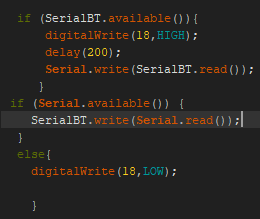
\includegraphics[height=5.0cm, width=6.0cm]{bluetooth}
	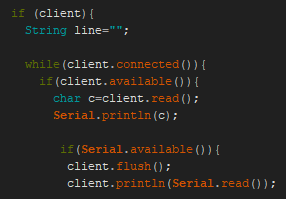
\includegraphics[height=5.0cm, width=6.0cm]{standard_wifi}
	\caption{Left: ESP32 Bluetooth main loop code.}
	\caption{Right: ESP32 standard Wifi main loop code.}
\end{figure}

Blynk is a library that when connected to its app on any mobile device provides a very aesthetic design for the user, it is also very customizable for varying project requirements.
The way it has been used in my case is of a similar procedure but is not as straightforward as the Bluetooth or standard WiFi set up. As you can see below, two functions are created with \verb|'BLYNK_WRITE'| being a Blynk library that reads commands from the mobile device and sends them to the Arduino and \verb|'SerialInput'| being the function which sends messages from the Arduino to the mobile device.

\begin{figure}[H]
	\centering
	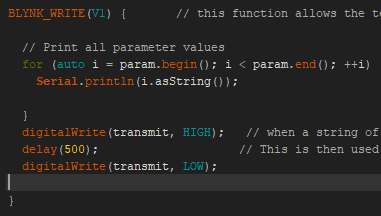
\includegraphics[height=5.0cm, width=6.0cm]{blynk1}
	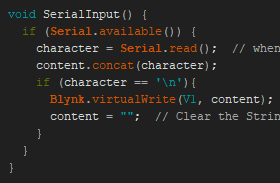
\includegraphics[height=5.0cm, width=6.0cm]{blynk2}
	\caption{Left: ESP32 Blynk read from the mobile device and send messages to the Arduino Mega.}
	\caption{Right: ESP32 Blynk read meaasges from arduino and send to mobile device}
\end{figure}

The ESP32 is a Dual core micro-controller and in theory can be used for a combined Bluetooth and WiFi mode. As you can see from the figure below this was attempted and does work, however there is one issue issues. Because the procedure for sending messages back to the mobile devices are virtually the same for WiFi and Bluetooth the ESP32 has no distinction between which device it has received a command from and therefore which device to send messages back to.

\begin{figure}[H]
	\centering
	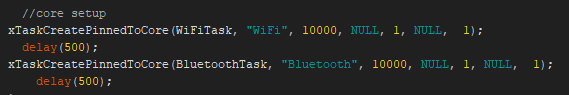
\includegraphics[height=4.0cm, width=15.0cm]{multicore}
	\caption{Setup for ESP32 dual core WiFi and Bluetooth.}
\end{figure}

Looking at the figure below you can see the main loop for the Arduino mega. The commands here are reading the serial monitor when the buggy is connected to the PC as well as the IR remote control reader and the ESP32 reader (this reads messages from the mobile device). Other commands that monitor the tilt sensor and the Wifi/Bluetooth connection are at the bottom of Figure 6. 

\begin{figure}[H]
\centering
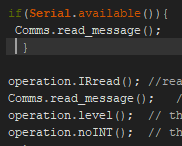
\includegraphics[]{main_loop}
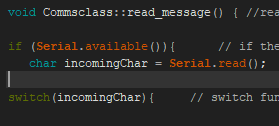
\includegraphics[height=4cm]{read_message}
\caption{Left: Arduino mega main loop}
\caption{Right: Read incoming message}
\end{figure}

When a command is received from the mobile device it will enter a \verb|switch| loop, here is where commands are executed. each command corresponds to a function which exist in other source code files.

\begin{figure}[H]
	\centering
	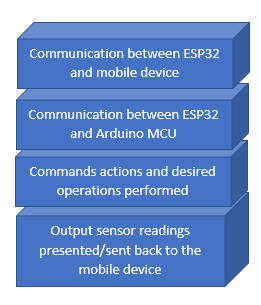
\includegraphics[]{layer}
	\caption{Layer diagram of the Buggies distributed system.}

\end{figure}

	///Layers- layered system to allow for easy maintenance, ease of updating/developing the system. ADD A DIAGRAM OF THE LAYERS HERE. 

\section{Testing}

The variety of testing methods used from start to finish have varied from unit and integration testing to acceptance and regression testing. The unit testing has taken place when a new operation/function has been added to the source code and is performed by myself for verification. The integration tests have then been performed by others to make sure that the new function works within the rest of the system and performs how it is expected to perform (acceptance testing). As the project has developed regression testing has been used to verify that any changes have not affected the prior system.   

One of the first problems discovered was with the ultrasound sensor (USS), in complex environments the USS would not recognise the correct distance and the buggy would therefore crash. Complex environments such as chair legs and/or approaching a wall at a 45$^{\circ}$ angle. The reason for the USS difficulty in getting the correct distances is due to its transmitter-receiver setup, if either one is blocked then the correct distance cannot be obtained and the buggy collides with the obstacle. For this reason, to reduce any damage to the hardware a tilt sensor was added. This feature when triggered will stop any movement of the buggy and will send a warning signal to the mobile device terminal. Initially the USS was fixed and when an obstacle was detected the buggy was set to turn left as a default. Since placing the USS on a servo motor it has become better at sensing obstacles and making decisions on which direction is best to move in before colliding with an obstacle. 

\begin{figure}[H]
	\centering
	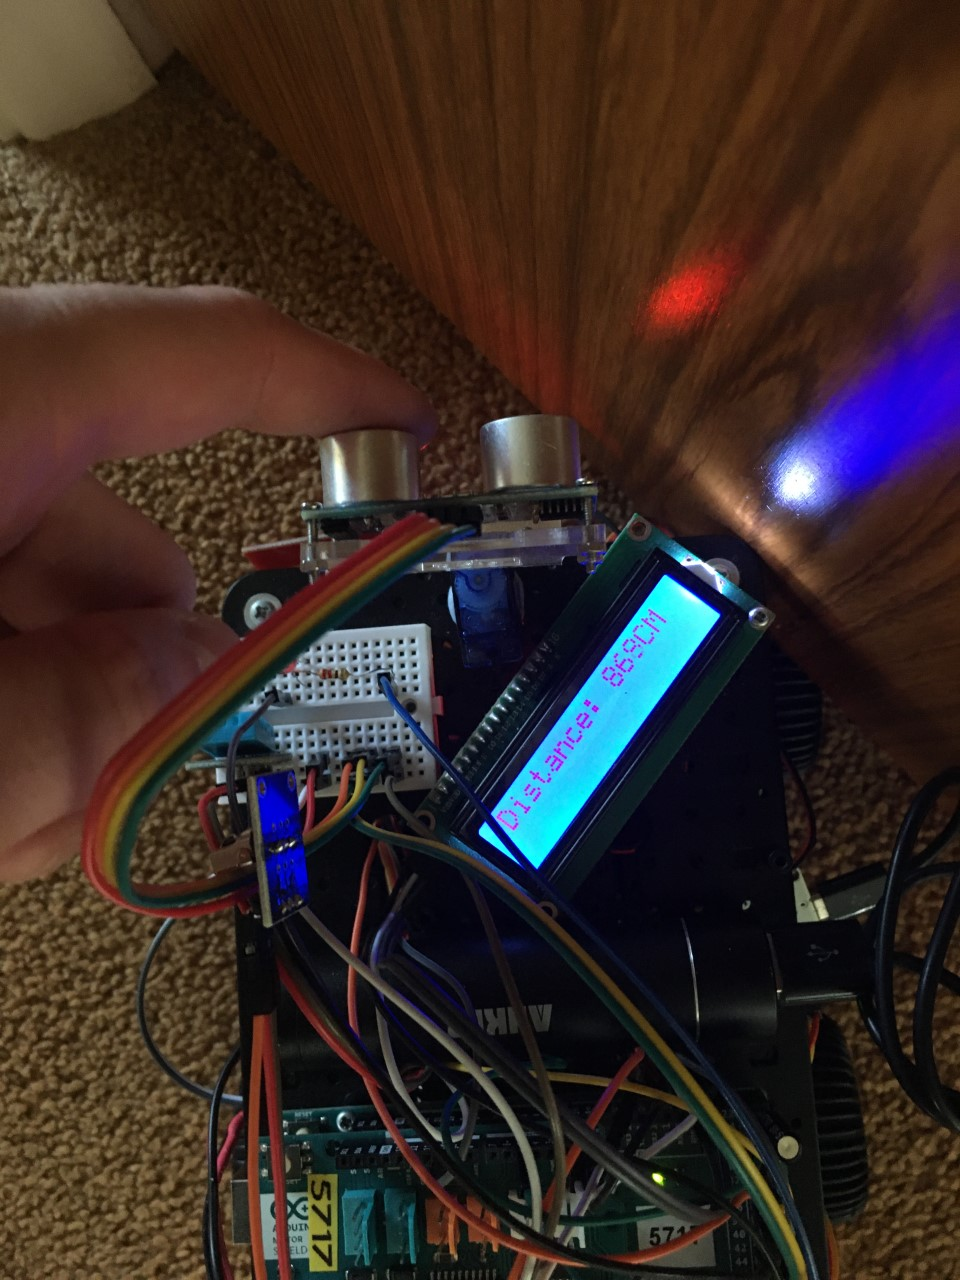
\includegraphics[height=5.0cm, width=4.0cm]{cover}
	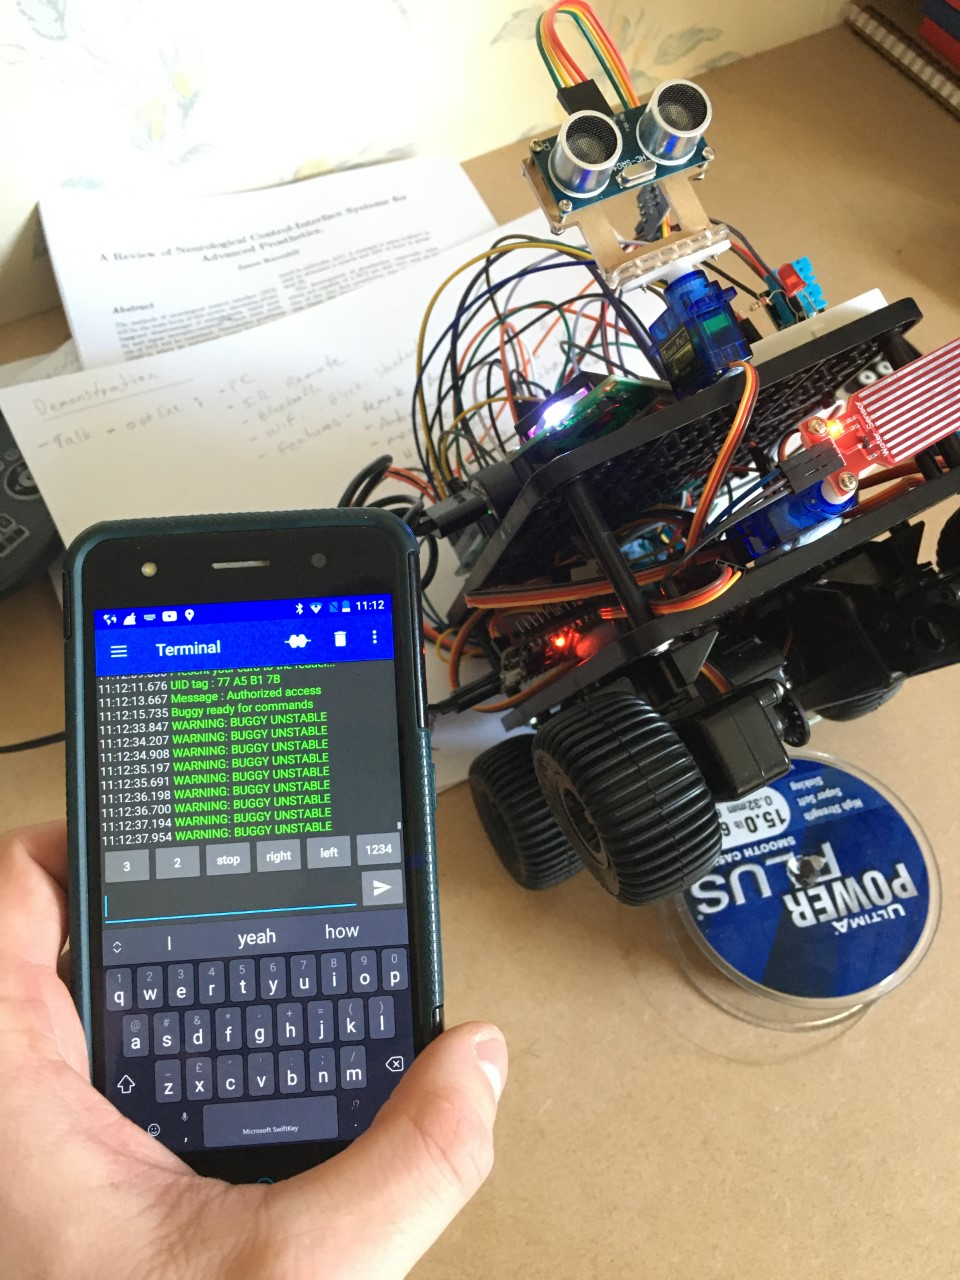
\includegraphics[height=5.0cm, width=4.0cm]{unstable}
	\caption{Left: Covering receiver/transmitter on approach to an obstacle and the USS showing a incorrect distance of 869CM.}
	\caption{Right: Unstable message displayed when buggy is tilted.}
\end{figure}

 
When the decision to add a IR remote which is able to control the buggy was made, initially there were issues. Noise from ambient light, other IR sources and even electrical signals within the breadboard caused overflow issues. Any command received from the IR remote would not be read and processed. 

What I found was happening is that any electrical signal to or from the ultrasound sensor was being spread throughout the pin ports in the breadboard (This is due to it being a small cheap breadboard) and this interfered with the IR LED electrical signal. To over come this the signal pin for the IR LED was relocated to the main Arduino mega board, This reduced the noise considerably.  


Of course loss of communication is a important problem. To combat this the ESP32 monitors WiFi/Bluetooth connection and if any connection is lost the ESP32 sends a signal to the Arduino Mega. This signal will stop the buggy and turn the front red LED light on. No message is sent to the mobile device as there is no connection so it would be pointless. When the connection is lost the LCD is also cleared. The ESP32 will attempt to restart the setup instructions to regain connection. 

\begin{figure}[H]
	\centering
	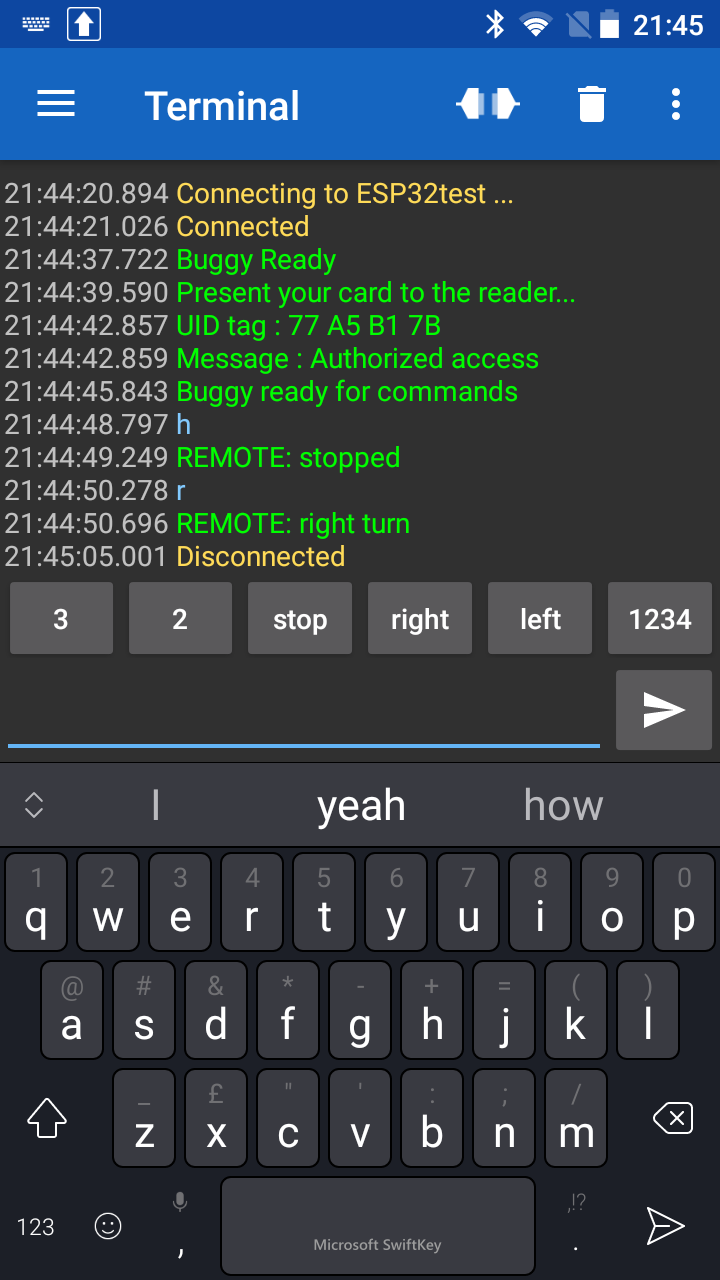
\includegraphics[height=5.0cm, width=4.0cm]{red_led_disconnect}
	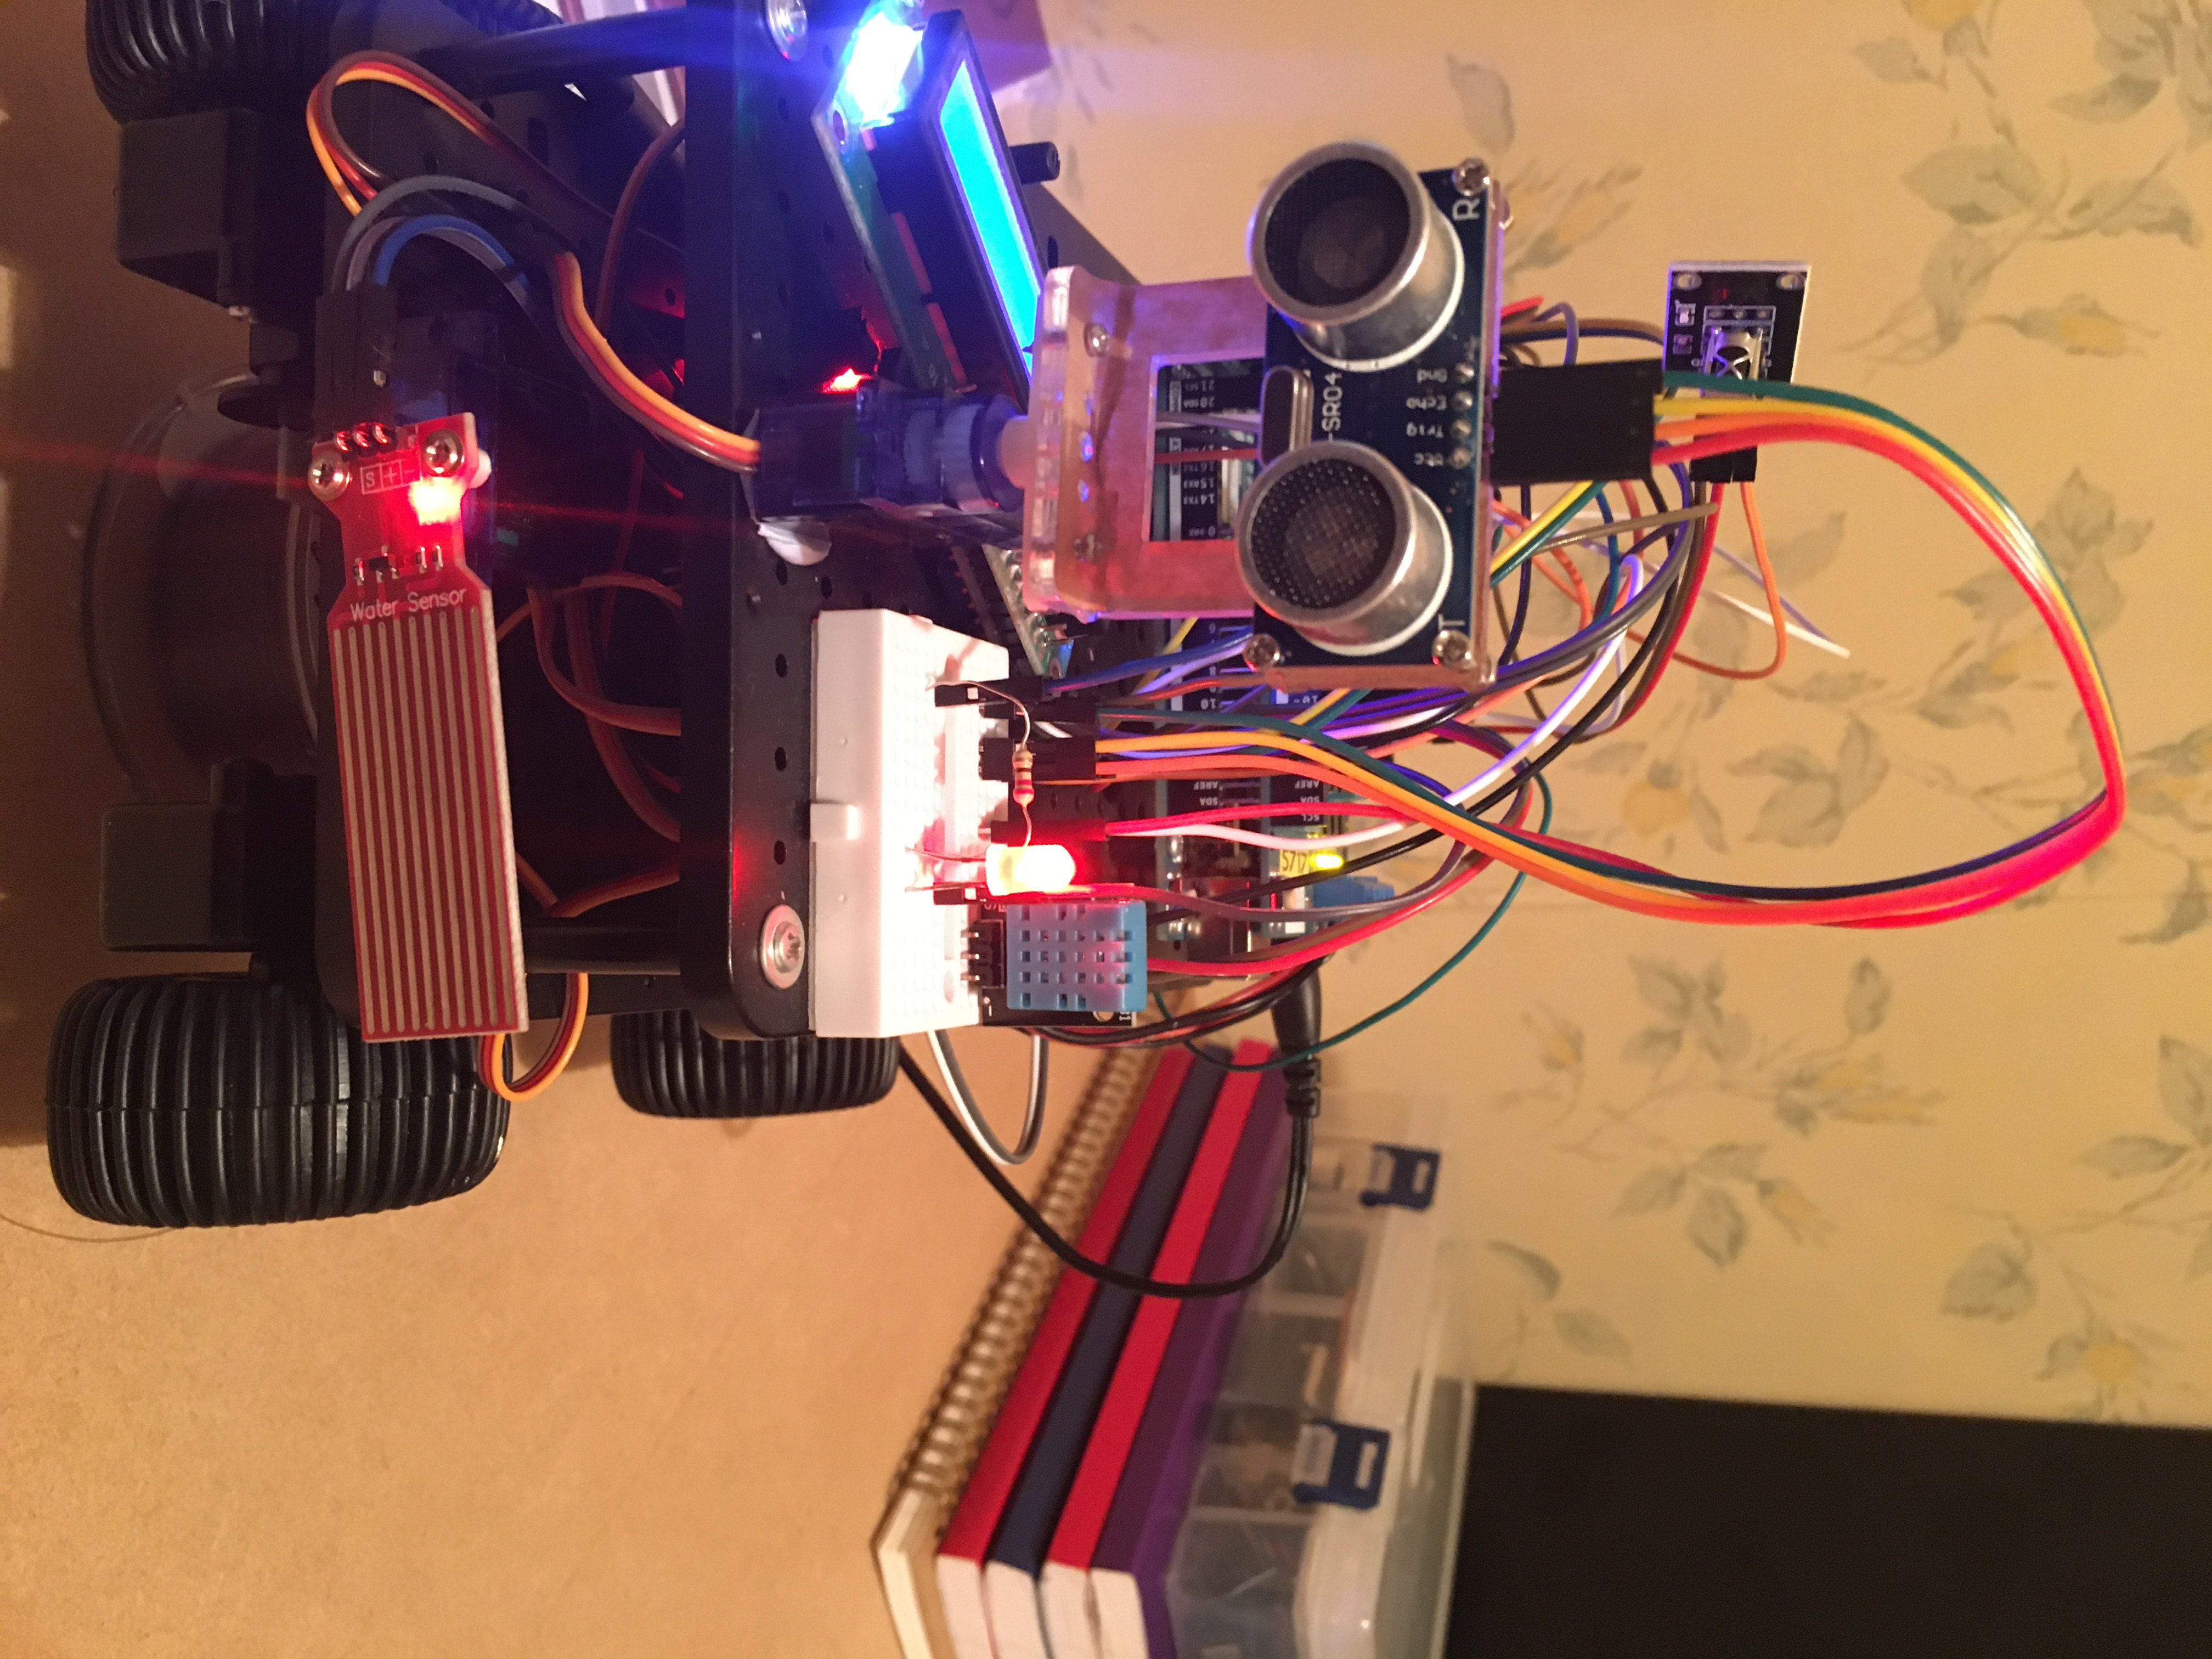
\includegraphics[height=5.0cm, width=4.0cm, angle=90, origin=c]{red_led}
	\caption{Left: Mobile device connecting and then disconnecting from the buggy.}
	\caption{Red LED on, after mobile device disconnects from buggy.}
\end{figure} 

Some basic tests on the accuracy of the ultrasound, temperature, humidity and water sensor were also conducted. When testing the accuracy of the ultrasound sensor a ruler was placed at the base of the sensor and a book was moved closer in intervals of 5cm starting from 5cm to 90cm. The recorded result was then noted and compared against the actual result. 

\begin{figure}[H]
	\centering
	\begin{tabular}{|c|c|c|}
		\hline
		Measured distance (cm) & Recorded distance (cm) & \verb|%| Error\\
		\hline
		 5 & 3 & 40 \\   
		 10 & 7 & 30\\
		 15 & 10 & 33 \\
		 20 & 14 & 30\\
		 25 & 17 & 32\\
		 30 & 21 & 30\\
		 35 & 23 & 34\\
		 40 & 27 & 33\\
		 45 & 30 & 33\\
		 50 & 34 & 32\\
		 55 & 37 & 33\\
		 60 & 41 & 32\\
		 65 & 44 & 32\\
 		 70 & 47 & 33\\
		 75 & 51 & 32\\
		 80 & 54 & 33\\
		 85 & 58 & 32\\
		 90 & 53 & 30\\
		\hline
	\end{tabular}
	\caption{Table of figures for ultrasound sensor test.}
\end{figure}

The \verb|%| error is relatively constant throughout which in our case isn't a bad thing, as it will allow me to calibrate the distance output by applying an offset of approximately 30 \verb|%|. This being said the ultrasound sensor still provides the buggy with efficient feedback of the distance from obstacles so no calibration will take place. Calibration will just remain an option if needed in the future.  




When It came to testing the temperature, ///////

The water sensor was slightly different when it came to testing. The software is setup to provide a ranged output for the sensor reading (Empty, low, medium and High). These ranges can be calibrated in the source code, but I still tested the sensor to see how the difference in water levels affected the output. The sensor was split up into intervals and water is applied in cumulative segments. The output is then recorded, the output can be recalibrated depending on how sensitive the user wants the sensor to be. 


\begin{figure}[H]
	\centering
	\begin{tabular}{|c|c|}
		\hline
		Depth submerged (cm) & Recorded output\\
		\hline
        0.0 & Empty\\
        0.5 & Low\\
        1.0 & Low\\
        1.5 & Medium\\
        2.0 & Medium\\
        2.5 & Medium\\
        3.0 & High\\
        3.5 & High\\
        4.0 & High\\
		\hline
	\end{tabular}
	\caption{Table of figures for water sensor test.}
\end{figure}
From the water sensor figures in the table above we can see that the water sensor is well calibrated for the situation of the buggy. As mentioned before the sensitivity of the water sensor can be changed in the source code by changing the analogue ranges for each corresponding level of empty, low, medium and high. 


\section{Evaluation}

There are some limitations to each method of distribution. When comparing the WiFi and Bluetooth methods when using the mobile device the Bluetooth is more favourable. This has been fed-back from the testing as well as personal experience. The WiFi and Bluetooth methods allow you to use the buggy to its full potential, however when it comes to usability the Bluetooth shines through. The reasons for this is that Bluetooth can be used anywhere and does not depend on a network connection like WiFi. The disconnection function is also instant when it come to using Bluetooth whereas there is a 10 second delay time for the buggy to realise it has disconnected from the local network when using the WiFi. 

Using the IR remote and PC are quite similar, they are both slightly limited as can not be used to stop the buggy from roaming around autonomously. This is due to the architecture of the source code. The buggy exits the autonomous mode when the ESP32 communicates to the Arduino, obviously because we are not using the ESP32 while using the IR remote or PC serial monitor then there is no way of signalling the Arduino to stop moving around autonomously. An attempt however was made so the IR remote would be able to signal the Arduino to exit its autonomous mode when a signal is received by the IR LED. Unfortunately because there is still some IR noise that exists in the external environment the buggy stopped roaming around autonomously when no such command was given. 

The difference in using the IR remote and a mobile device is great. When you are using the mobile device, you can control to buggy from a different room if you wanted to, whereas the user is unable to do this with the IR remote. The IR remote can however be used simultaneously with a mobile device, so two people can control the buggy at the same time. This is useful as if there is an issue with the IR remote then the buggy can still be controlled with the mobile device or visa versa. 

When using the buggy in a Bluetooth mode, two devices can not be connected to the buggy. However when using the dual-core capability of the ESP32 (with one core setup using WiFi and the other Bluetooth) two mobile devices can be connected. This works well however, any messages sent back to the mobile devices from the buggy can get scrambled. This means that if the first mobile device sends a command to the buggy, the returning message will be delivered to the other device. There are positives and negatives for this. One positive is that it allows the other user to know what is happening with the buggy but the one that issues the command does not know if the command has been executed other than by physically watching the buggy. 

As you can see below when a command is sent from the Bluetooth terminal any messages responding to this command come back through the WiFi terminal and visa versa. 
	
	\begin{figure}[H]
		\centering
		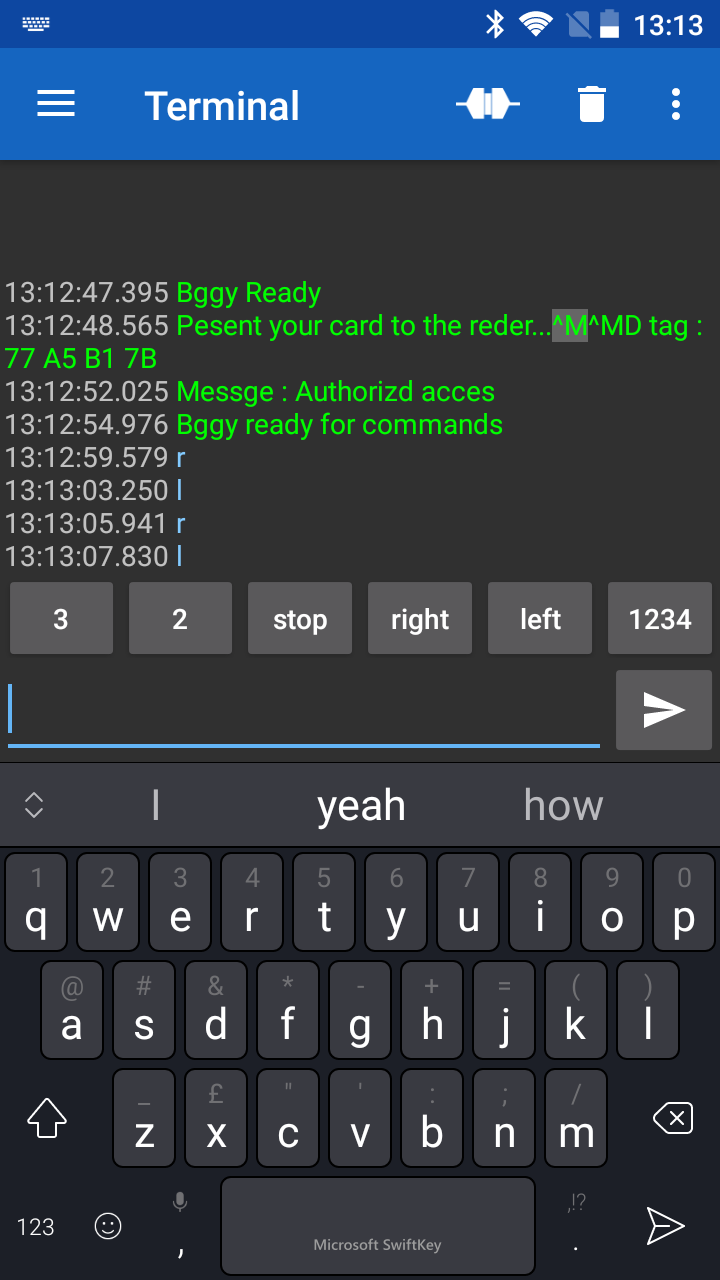
\includegraphics[height=5.0cm, width=4.0cm]{BLE_term}
		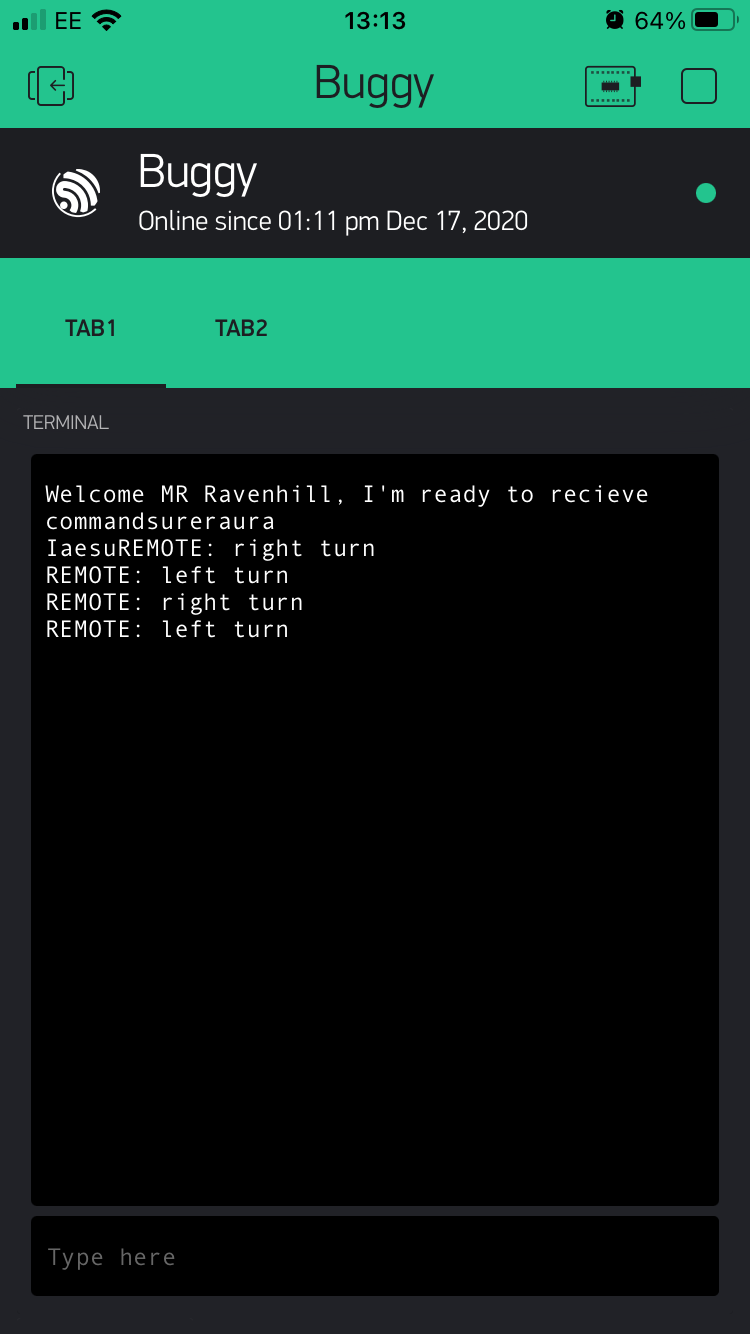
\includegraphics[height=5.0cm, width=4.0cm]{blynk_term2}
		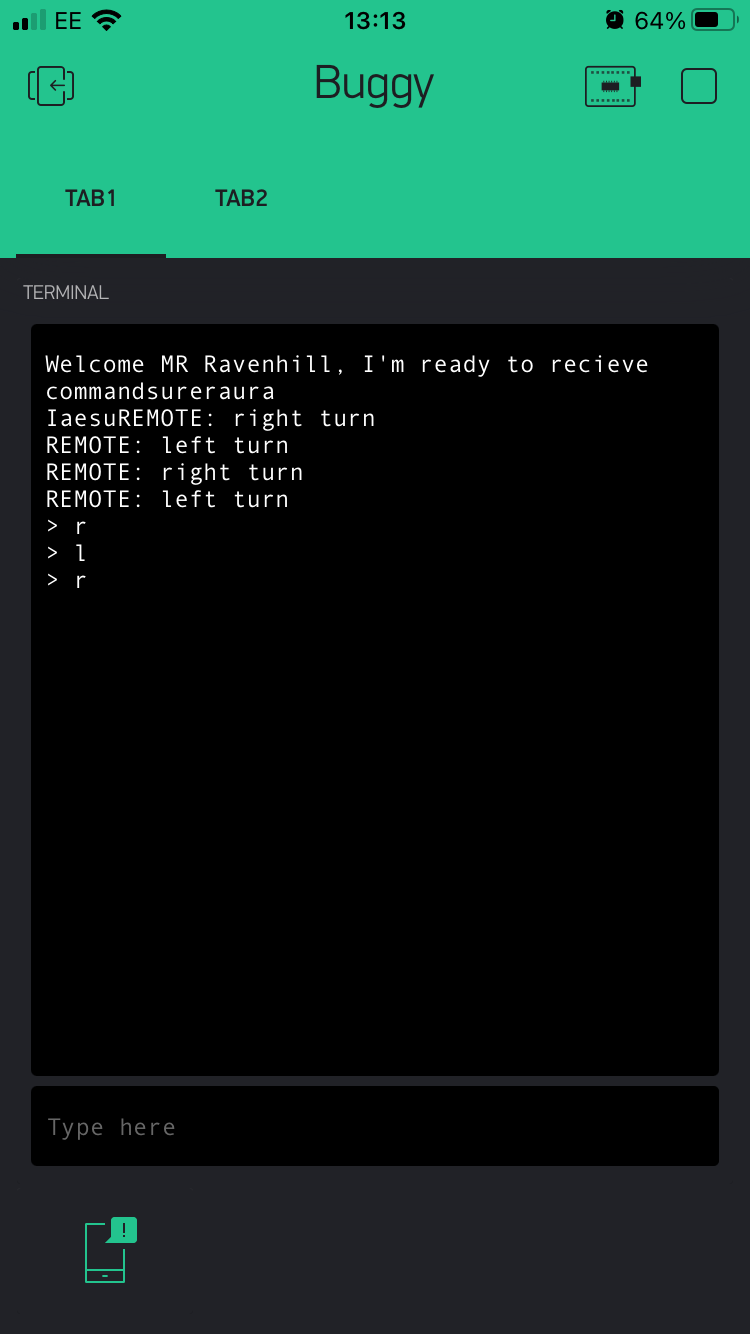
\includegraphics[height=5.0cm, width=4.0cm]{blynk_term}
		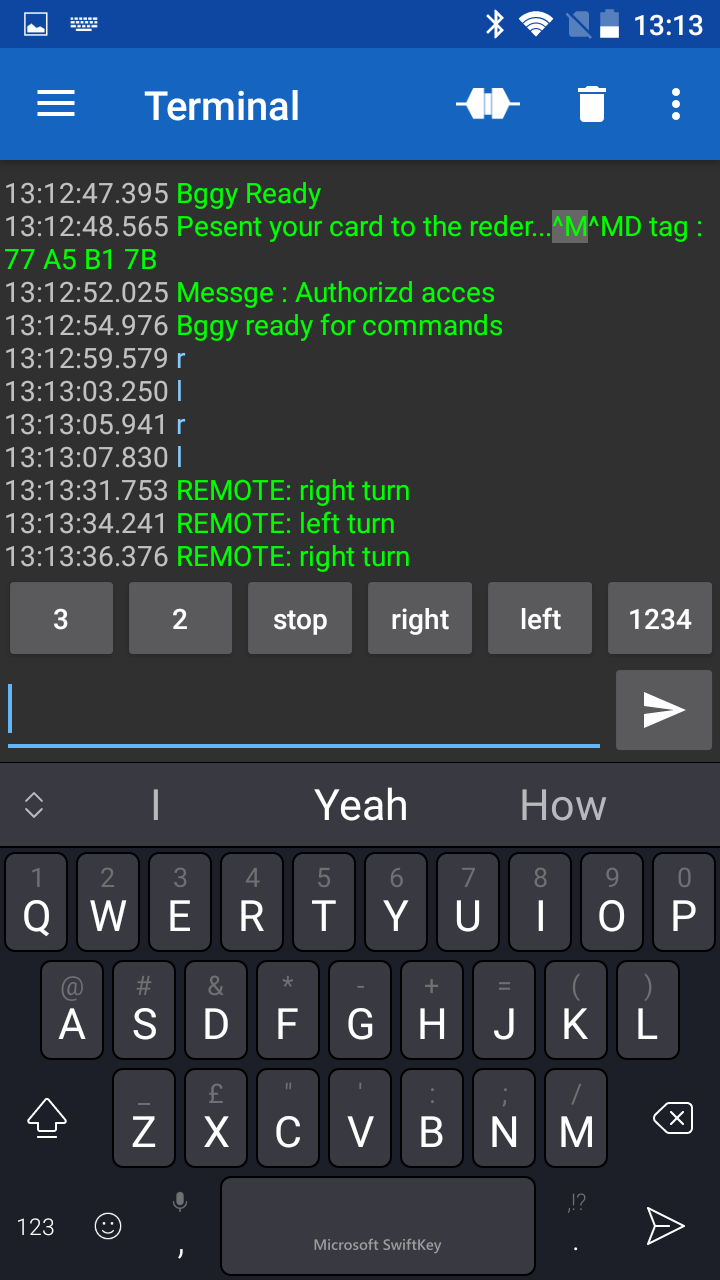
\includegraphics[height=5.0cm, width=4.0cm]{BLE_term2}
		\caption{From Left to Right: Bluetooth terminal giving commands. WiFi terminal receiving messages. WiFi terminal sending commands. Bluetooth terminal receiving messages.}			
	\end{figure}
	

	

\section{Code quality/remarks}






\section{Conclusion}


\section{Reference Library and appendices}
\subsection{Github account}

\href{https://github.com/james8268/Buggy}{Click here for Github hyper link} 

or copy and paste the URL into your web browser. https://github.com/james8268/Buggy

\listoffigures

\subsection{Third party libraries}

\verb|arduino.h|, \verb|LiquidCrystal_I2C.h|, \verb|IRremote.h|, \verb|Wire.h|, \verb|dht.h|, \verb|SPI.h|, \verb|MFRC522.h|, \verb|WiFi.h|, \verb|WiFiClient.h|, \verb|BlynkSimpleEsp32.h|, \verb|Servo.h| and \verb|BluetoothSerial.h|



\subsection{Test Comments}
Test 1

Getting to grips with the Bluetooth, 28/10/2020: The device worked exactly how it should every command button worked as it should. The controls were very easy to understand and get to grips with which means I could use the buggy how I wanted with no issues. Only thing I would like to add is that the left and right turns be a little less aggressive. So instead of a 90 degree turn maybe a 45 instead. Also I would like the distance of the sensor to be displayed on the mobile device as well as the LCD screen on the buggy so I don’t have to be stood directly over the buggy to know this information, as I think this would make it more user friendly. Other than that, it was flawless.

Test 2

This test is like the last with a few minor changes. This time around the buggy is in a combined remote Bluetooth and autonomous mode. The autonomous element will allow the buggy to roam freely while avoiding obstacles.

Acting on the previous test a feature of being able to see the reading of the ultrasound sensor has now been added and can be viewed in the mobile device terminal as well as the turns being less harsh.

Test 2.1, using the combined autonomous and Bluetooth mode, 04/11/2020: self-roaming was effective, the buggy avoided obstacles well, although had trouble once it was under a certain distance from complex obstacles. commands were easy to pick up and the buggy was easy to manoeuvre, although lag time could be reduced, or possibly a cut off after x number of commands. possibly introduce a short cut to speed one and/or options for varying stop times, so that when flustered a driver can take time to re-think.

Test 2.2, test is the same as previous (code remains the same as the last test), 05/11/2020: the buggy avoided the obstacles well however due to lag it made it difficult to manoeuvre, also would be much easier and efficient for the driver if there was a cut off command so that the user can re-access the situation and move from there.  

Test 3

The buggy now can roam around autonomously while avoiding obstacles and this can then be stopped and be used remotely again. It’s easy to switch between the two, using the mobile device terminal the "roam" hotkey enters the buggy into an autonomous mode(which can be seen when the android device is tilted on a landscape view and the screen will show more potential hotkeys). when any button/command is used in the terminal the buggy will then exit the autonomous mode and reverts to a remote mode. 

Test 3, testing combined autonomous and remote modes, 07/11/2020: I enjoyed the new features on the handset. The fact that the buggy now had a roam feature was very interesting. The fact it could now make decisions on what was in front of it and change the course on which it was travelling due to an object being in its way was fascinating. A cool feature would be if it could decide which way it wanted to turn. For instance, left or right depending on the amount of space it has either side, this depends on the amount ultrasound sensors it has available. All the other buttons worked well and did what I wanted when I asked it to. 

Test 4

A tilt sensor and servo motor have now been added, the use of WIFI connection is also up and running. Security measures have been added so if WIFI or Bluetooth connection is lost it will stop the buggy and turn on the front red LED. The servo motor allows the buggy to look left and right and then decide on which direction to move. The tilt sensor will monitor the buggy and if it capsizes or is flipped over it will stop the buggy and turn on a buzzer as well as notifying the user if in remote mode. 

tests to be completed:
\begin{itemize}
\item turning system for servo ultrasound sensor, just to check its working right.
\item tilt sensor while in autonomous mode while moving. 
\item temp and humidity sensor and water sensor while moving and stationary. 
\item disconnect functions via Bluetooth, by trying to connect another device (already known that two devices can’t connect over Bluetooth).
\item disconnect from WiFi, turn off router. 
\item test overall usability.
\end{itemize}

Test 4, 23/11/2020, testing the new obstacle avoidance system, tilt sensor and the temp, humidity and water sensor (all in Bluetooth mode): I found the new obstacle avoidance system was very good the Buggy made very accurate adjustments when it came to an obstruction. the fact it was able to stop look around and decide for itself which way to go was very impressive. the tilt sensor that has been integrated into the buggy was a very impressive feature. especially since you had the use of this both in autonomous mode and just when controlling the buggy, yourself. also having the bonus of a water, temp and humidity sensor on it was very good. being able to see those readings was a nice feature to have the use of. I also found the use of the IR remote to be far more simplistic and easier to use than the Bluetooth device I much preferred it. there was a few points I feel could do with some improvement. for instance, when you are on the move and then ask the buggy to perform a water reading it stops does this command but then waits for another new instructions. I would like it to instantly carry on with the previous command once the reading has been carried out with no need to give it further instruction from either the Bluetooth device or IR remote. other than that, the buggy was very good.

Test 5

A RFID security tag has been added for security. 

Test 5, first time using WIFI set up and looking at disconnection issues. To then compare the WIFI and Bluetooth usability, 11/12/20: 

Using BLYNK: was detailed and easy to use. Very easy to read the screen. All commands worked straight away. Liked the safety feature as well the fact you had to use a key fob to be able to use the buggy. Also, the fact it tells you on the buggy with a red led that it is disconnected from the internet and you no longer have control of the buggy. 

Standard WIFI:  wasn’t as easy to use. Didn’t like the fact every time you placed a command the keyboard went away so you had to click on the box again to load a command. When I asked for a temp reading it wasn’t displayed on the WIFI app. Just gave me a random number. Also, when disconnected from the internet the red led light didn’t show on the buggy to indicate it was inoperable, however it did show on the WIFI app that it had been disconnected from the network.  

Comparison to Bluetooth: WIFI was good but the Bluetooth was far better in my opinion as I can used the buggy anywhere at any time I like with ease. Whereas with the WIFI you must have that connected to be able to use the buggy. Also, the Bluetooth has the hot keys which made the whole experience of using the buggy more user friendly and easier. 



\end{document}